\begin{figure}[h]
  \centering
  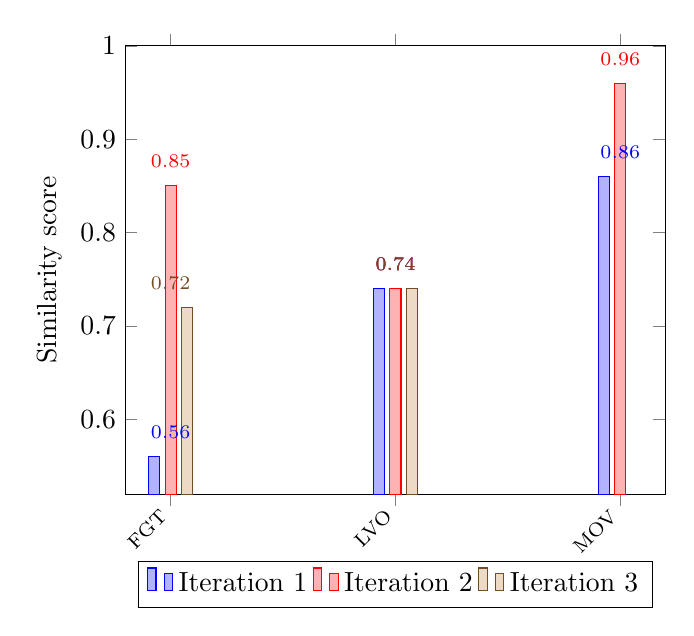
\begin{tikzpicture}
    \begin{axis}[
        ybar,
        bar width=4pt,
        enlargelimits=0.1,
        ylabel={Similarity score},
        symbolic x coords={FGT, LVO, MOV},
        xtick=data,
        x tick label style={rotate=45, anchor=east, font=\scriptsize},
        nodes near coords,
        point meta=y,
        nodes near coords align={vertical},
        every node near coord/.append style={font=\scriptsize},
        every node near coord/.append style={
          /pgfplots/bar shift=0pt,
          shift={(0pt,3pt)}
        },
        legend style={at={(0.5,-0.15)}, anchor=north, legend columns=-1}
    ]
      % Iteration 1
      \addplot coordinates {(FGT,0.56) (LVO,0.74) (MOV,0.86)};
      % Iteration 2
      \addplot coordinates {(FGT,0.85) (LVO,0.74) (MOV,0.96)};
      % Iteration 3
      \addplot coordinates {(FGT,0.72) (LVO,0.74)};
      \legend{Iteration 1, Iteration 2, Iteration 3}
    \end{axis}
  \end{tikzpicture}

  \caption{Similarity scores for the HAR case study across 3 iterations.}
  \textbf{Abbreviations:}
  \caption*{\footnotesize
  \begin{tabular}{@{}ll@{\hspace{1cm}}ll@{}}
  FGT & Fighting & MOV & Moving \\
  LVO & Leaving Object &  &  \\
  \end{tabular}
  }

  \label{fig:iteration_scores}
\end{figure}